\documentclass{exam}
\usepackage{amssymb}
\usepackage{lipsum} 
\usepackage{graphicx}
\usepackage[
backend=biber
]{biblatex}
\addbibresource{refs.bib}

\usepackage{hyperref}
\hypersetup{
    colorlinks=true,
    linkcolor=blue,
    citecolor=black,
    filecolor=blue,      
    urlcolor=blue,
}

\newcommand\labnr{9}
\newcommand\lab{Lab \labnr\ - Minimum Spanning Trees}

\newcommand\uni{Technical University of Cluj-Napoca}
\newcommand\course{Data Structures \& Algorithms}

\newcommand\lvlez{$\bigstar$}
\newcommand\lvlmed{\lvlez\lvlez}
\newcommand\lvlhard{\lvlmed\lvlez}
\newcommand\lvlvhard{\lvlhard\lvlez}


\pagestyle{headandfoot}
\firstpageheader{}{}{}
\firstpagefootrule
\firstpageheadrule
\firstpagefooter{\sc\uni}{}{\sc\course, Lab \labnr}
\runningheader{\sc\uni}{}{\sc\course, Lab \labnr}
\runningheadrule
\runningfootrule
\runningfooter{}{\thepage}{}

\usepackage{listings}
\usepackage{xcolor}
\usepackage{svg}

\definecolor{codegreen}{rgb}{0,0.6,0}
\definecolor{codegray}{rgb}{0.5,0.5,0.5}
\definecolor{codepurple}{rgb}{0.58,0,0.82}
\definecolor{backcolour}{rgb}{0.95,0.95,0.92}

\lstdefinestyle{mystyle}{
    commentstyle=\color{codegreen},
    keywordstyle=\color{magenta},
    stringstyle=\color{codepurple},
    basicstyle=\ttfamily\footnotesize,
    breakatwhitespace=false,         
    breaklines=true,                 
    captionpos=b,                    
    keepspaces=true,                 
    showspaces=false,                
    showstringspaces=false,
    showtabs=false,                  
    tabsize=2
}
\lstset{style=mystyle}

\begin{document}
\begin{center}
    \vspace*{0cm}
    \bfseries\LARGE
    \lab
    \vspace*{1cm}
\end{center}


\begin{questions}
\question Implement Kruskal's algorithm using any graph representation you want: \cite{cormen2022introduction}

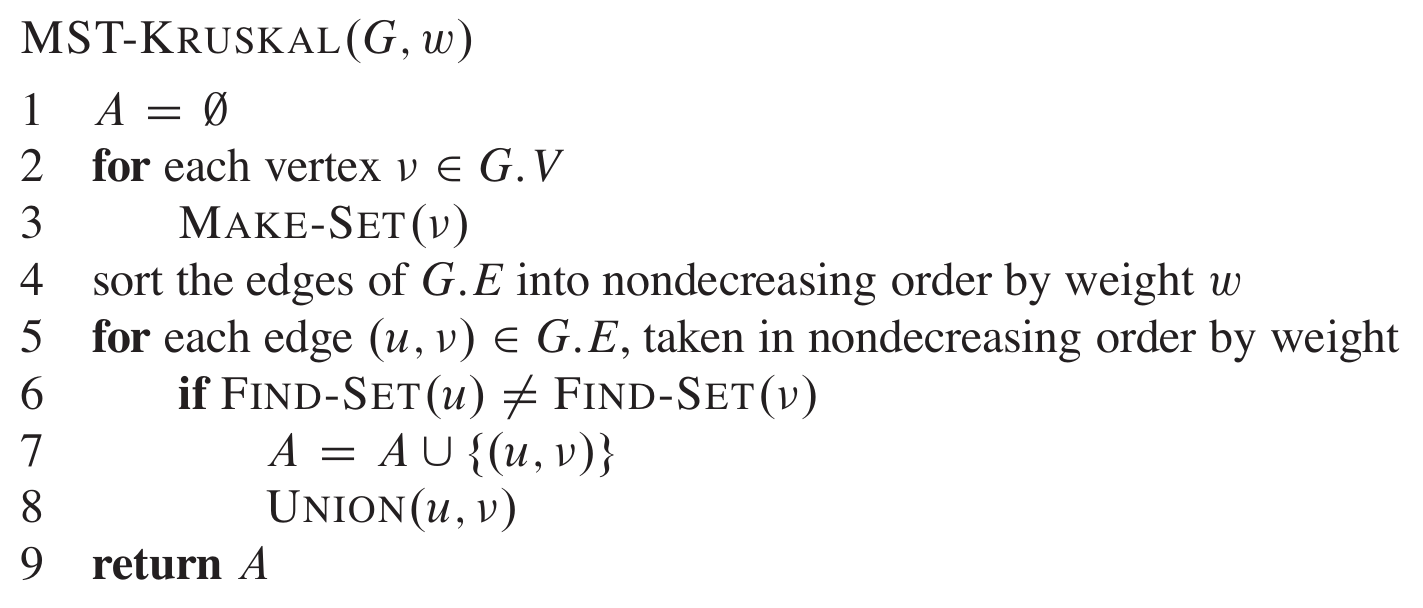
\includegraphics[width=0.6\textwidth]{diagrams/kruskal.png}



\question Implement Prim's algorithm using any graph representation you want: \cite{cormen2022introduction}

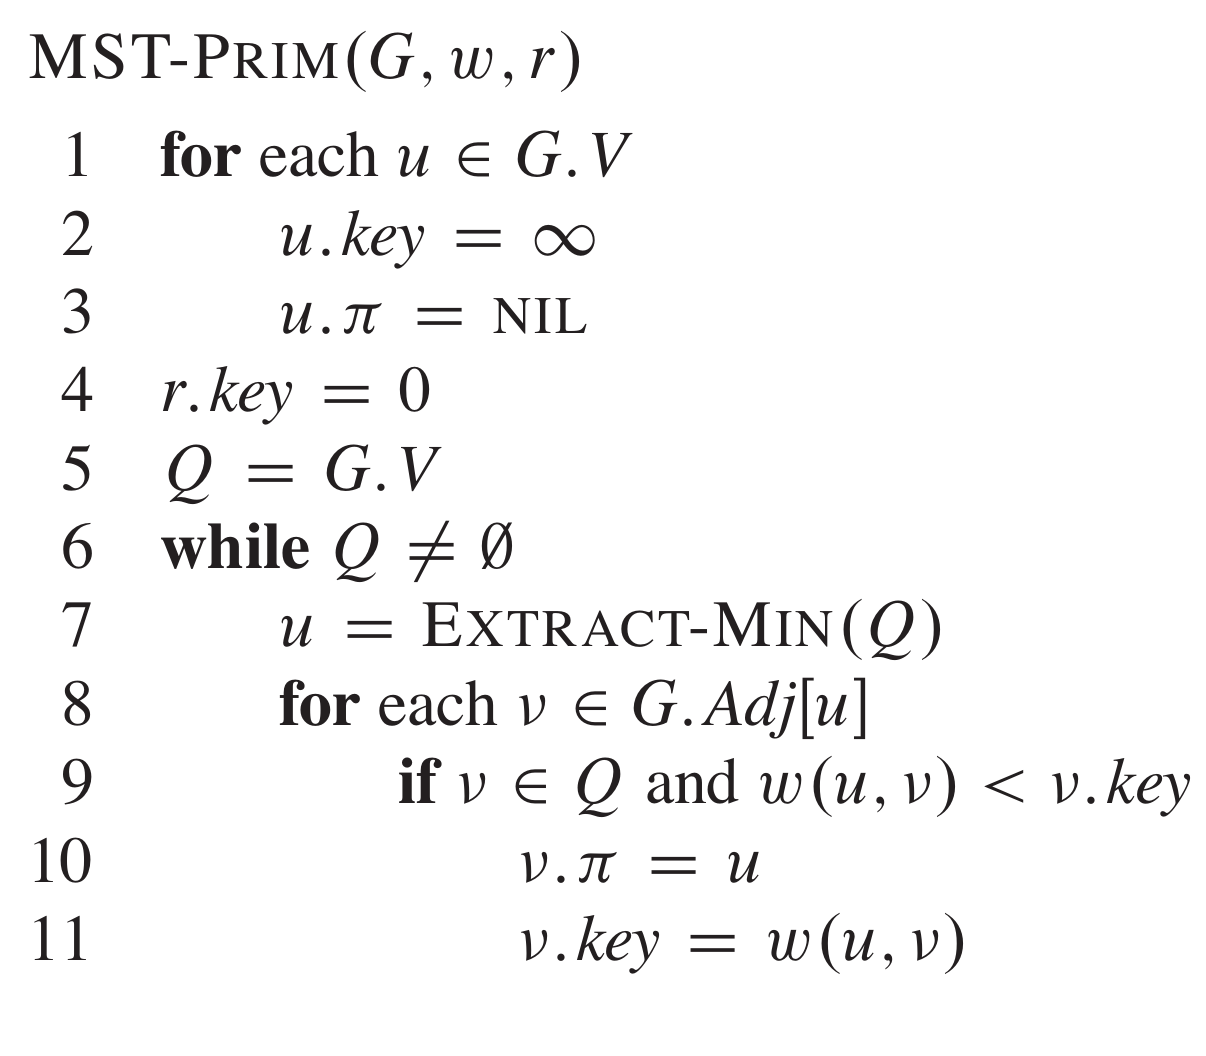
\includegraphics[width=0.38\textwidth]{diagrams/prim.png}

\end{questions}

 \bigskip
\textbf{Note:} Leave a comment with the text PB1, PB2.A.II, ... PB10 above every function that implements the respective lab task. (upper case text, no space between the text and the problem number)

\medskip
\printbibliography
\end{document}
